% -------------------------------------------------------------------------------
% This is all preamble stuff that you don't have to worry about.
% Head down to where it says "Enter your name here"
% -------------------------------------------------------------------------------
 
\documentclass[12pt]{article}
 
\usepackage[margin=1in]{geometry} 
\usepackage{amsmath,amsthm,amssymb}
\usepackage{graphicx}
\usepackage{enumerate}
\usepackage[names]{xcolor}
\usepackage{wrapfig}
\usepackage[multiple,hang,flushmargin]{footmisc}

\usepackage[parfill]{parskip}
\parskip=\baselineskip

 
\newenvironment{question}[2][Question]{\begin{trivlist}
\item[\hskip \labelsep {\bfseries #1}\hskip \labelsep {\bfseries #2.}]}{\end{trivlist}}
\newenvironment{solution}[1][Solution:]{\begin{trivlist}
\item[\hskip \labelsep {\bfseries #1}\hskip \labelsep {\bfseries}]\color{blue}}{\end{trivlist}}

\usepackage{fancyhdr}
\pagestyle{fancy}
\rhead{Due: \duedate}
\lhead{CSC250 - Final Examination}
\cfoot{p. \thepage}
\renewcommand{\headrulewidth}{0.4pt}
\renewcommand{\footrulewidth}{0.4pt}

 \makeatletter
\renewcommand\footnotesize{%
   \@setfontsize\footnotesize\@ixpt{11}%
   \abovedisplayskip 8\p@ \@plus2\p@ \@minus4\p@
   \abovedisplayshortskip \z@ \@plus\p@
   \belowdisplayshortskip 4\p@ \@plus2\p@ \@minus2\p@
   \def\@listi{\leftmargin\leftmargini
               \topsep 4\p@ \@plus2\p@ \@minus2\p@
               \parsep 2\p@ \@plus\p@ \@minus\p@
               \itemsep \parsep}%
   \belowdisplayskip \abovedisplayskip
}
\makeatother

\begin{document}
\newcommand{\duedate}{05/10/24 by 2:00pm EST}
 

% --------------------------------------------------------------------------------------------
%  Great, now skip ahead to where you see *** START EXAM HERE ***
% --------------------------------------------------------------------------------------------

\topskip0pt
\vspace*{\fill}
\begin{center}
\fbox{\fbox{\parbox{5.5in}{\begin{center}
\vspace{1em}
This is the second of two examinations for\\ \textbf{CSC250: Theory of Computation}\\ as taught by R. Jordan Crouser and Pablo Frank in Spring 2024.\\
\vspace{1em}
This exam is \textbf{open book and open note}.\\ The following materials are \textbf{permitted} while taking this examination:
\vspace{1em}
\begin{itemize}
	\item your own notes
	\item lecture slides / videos
	\item scribe notes
	\item homework solutions
	\item any of the recommended textbooks
\end{itemize}
\vspace{1em}
\textbf{Honor code: no other resources are permitted during this exam.}\\
This includes (but is not limited to): online materials, tutors, teaching assistants, and other students.
\end{center}
\vspace{5em}
 \ \ \ YOUR NAME: \underline{\hspace{10cm}}
\vspace{3em}}}}
\end{center}
\vspace{3em}
\vspace*{\fill}


% ---------------------------------------
%   *** START EXAM HERE ***
% ---------------------------------------

% -------------------------
% Regular languages
% -------------------------
\clearpage
\begin{question}{0}\textbf{Getting in the Groove}
\begin{center}
\textit{Note: This question is optional, but strongly recommended.}
\end{center}
Educational research studies\footnote{Lang, Jonas WB, and Jessica Lang. ``Priming competence diminishes the link between cognitive test anxiety and test performance: Implications for the interpretation of test scores.'' \textit{Psychological Science} 21.6 (2010): 811-819.}\footnote{Barrows, Jennifer, Samantha Dunn, and Carrie A. Lloyd. ``Anxiety, self-efficacy, and college exam grades.'' \textit{Universal Journal of Educational Research} 1.3 (2013): 204-208.} have suggested that people perform better on tests when they spend a few minutes thinking about things they're good at before they begin.\\\\
In the space below, briefly tell us about a time when you were \textbf{really successful} at doing something challenging (it doesn't have to be related to this course). If you prefer, you can draw a picture instead of writing.
\vfill
\hfill

\includegraphics[width=3in]{youcandoit-zoom.jpg}
\end{question}
\clearpage

% -------------------------
% Regular languages
% -------------------------
\begin{question}{1}\textbf{The Computational Hierarchy} (12 points)\\\\
On the following diagram, label each of the following complexity classes and give an\\example of a language in each class. You \textbf{do not} need to reproduce the proof.
\begin{center}
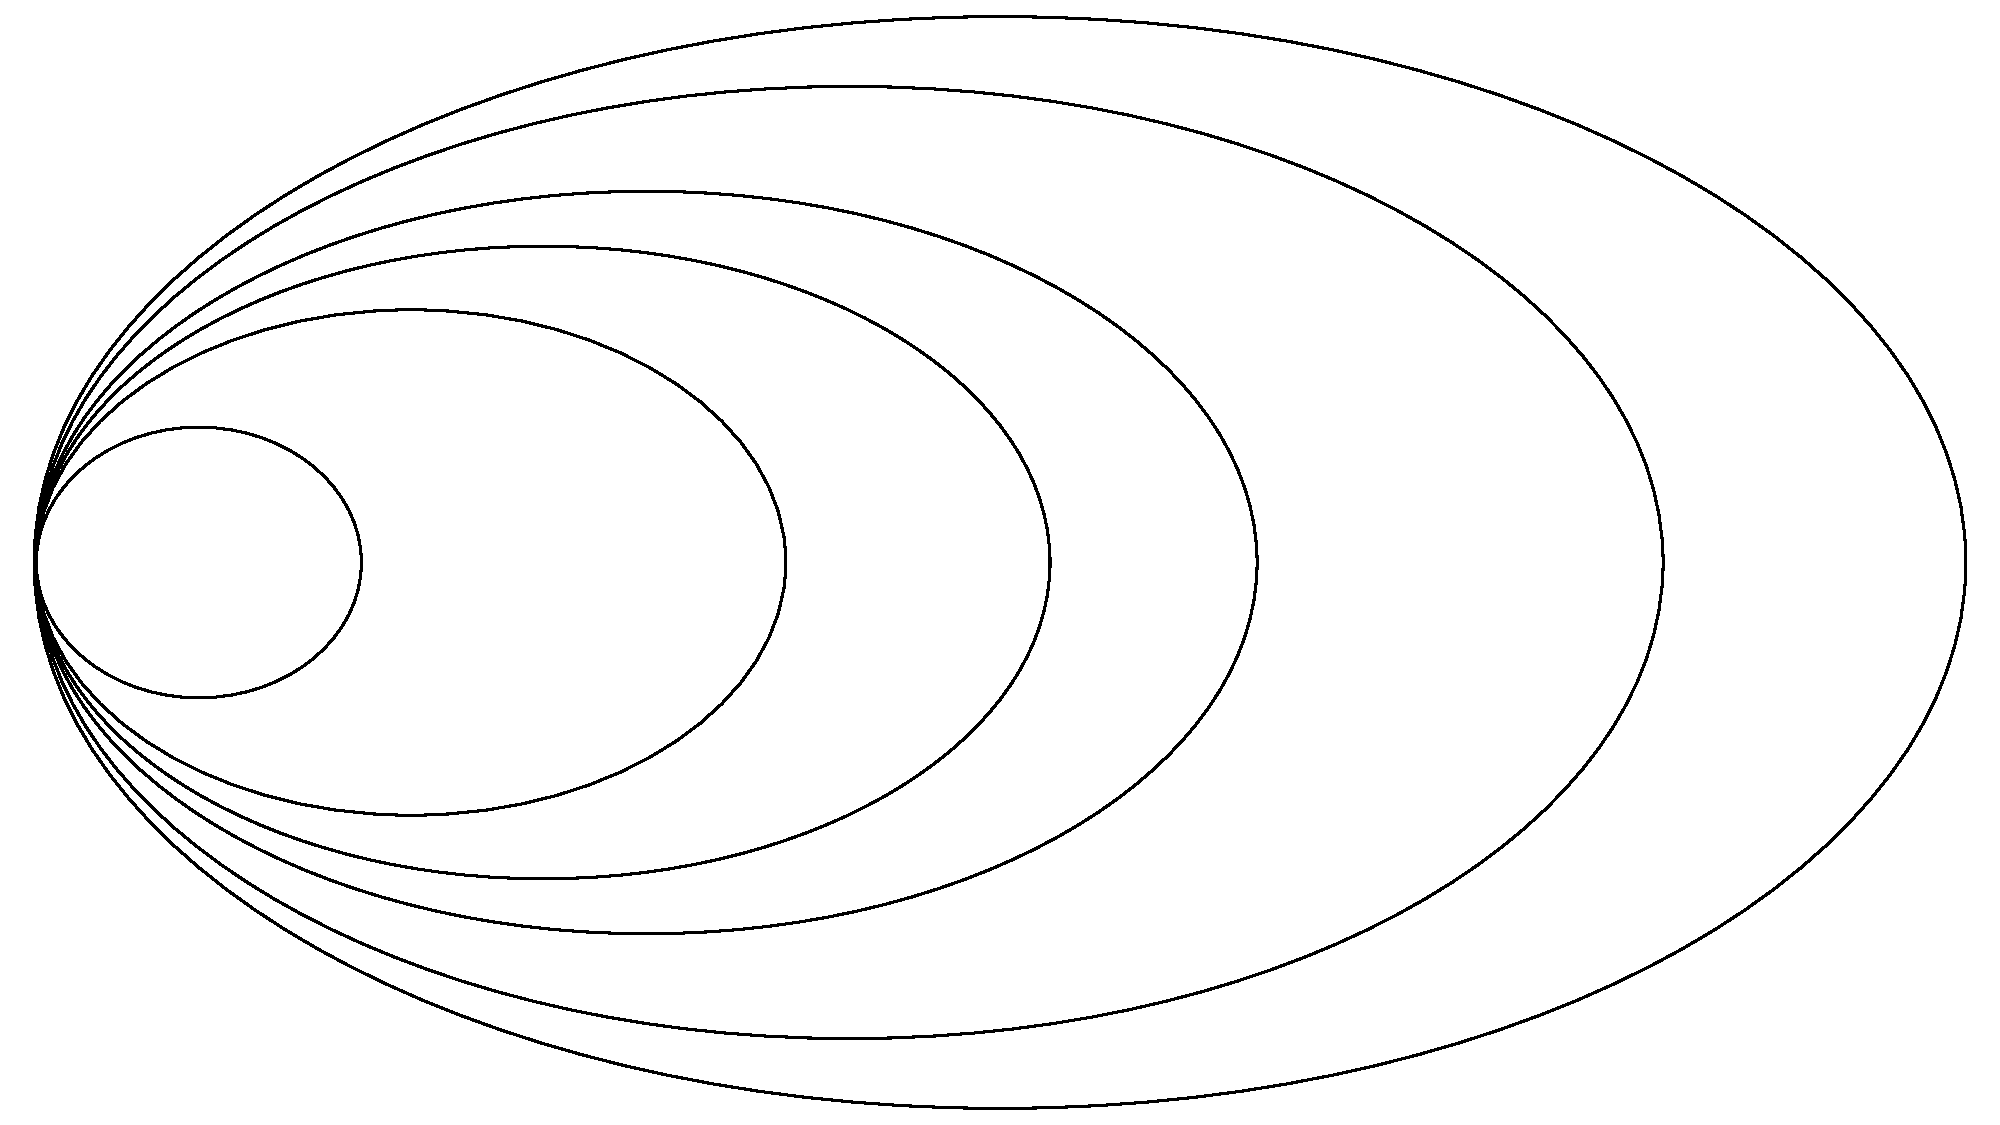
\includegraphics[width=0.9\textwidth]{diagram.pdf}
\end{center}
\begin{enumerate}[(a)]
	\setlength{\itemsep}{2em}
	\item Decidable languages
	\item Recognizable languages
	\item Context-free languages
	\item Regular languages
	\item $\mathcal{P}$
	\item $\mathcal{NP}$
\end{enumerate}
\end{question}
\clearpage

% -------------------------
% Regular languages
% -------------------------
\begin{question}{2}\textbf{Regular languages} (3 points) \\\\
Prove that the following language is regular: \[NOTBLANK = \{w \ | \ w \texttt{ is any binary string except the empty string}\}\]
\end{question}
\clearpage


% -------------------------------
% Non-regular languages
% -------------------------------
\begin{question}{3}\textbf{Non-regular languages} (6 points)\\\\
Prove that the following language is \textbf{not} regular: \[NOTPAL = \{w \ | \ w \not = w^R \ \texttt{(that is, } w \texttt{ is not a palindrome)}\}\]
\end{question}

\clearpage


% -------------------
% Undecidability
% -------------------
\begin{question}{4}\textbf{Undecidable languages} (6 points)\\\\
Consider the problem of trying to determine whether a Turing machine $M$ accepts only palindromes.
\begin{enumerate}[(a)]
\item Formulate this problem as a language.\\\\\\\\
\textit{JUST-PALS =}\hfill
\vspace{4em}
\item Show that this language is \textbf{undecidable}.
\end{enumerate}
\end{question}

\clearpage

% ----------------------
% Unrecognizability
% -----------------------
\begin{question}{5}\textbf{Unrecognizable languages} (4 points)\\\\
Show that the following language is \textbf{unrecognizable}:
\[LOOKS-FAMILIAR = \{\langle M,w\rangle \ | \ M \texttt{ does not accept } w\}\]
\end{question}
\clearpage

% ---------------
% Reductions
% ---------------
\begin{question}{6}\textbf{Reductions} (6 points)\\\\
Describe the key characteristics each of the following types of reductions. If they're useful for particular kinds of proofs, which ones? If they have shortcomings, note them. 
\begin{enumerate}[(a)]
	\item $\le_T$ 
	\vspace{12em}
	
	\item $\le_m$ 
	\vspace{12em}
	
	\item $\le_p$ 
	
	
\end{enumerate}
\end{question}

% ---------------
% P
% ---------------
\clearpage
\begin{question}{7}\textbf{$\mathcal{P}$} (6 points)\\\\
A \textbf{triangle} in an undirected graph is a 3-clique.
\begin{enumerate}[(a)]
\item Draw a graph that contains at least one triangle.
\vspace{10em}	
\item Show that $TRIANGLE = \{\langle G \rangle \ | \ G \texttt{ contains at least one triangle}\} \in \mathcal{P}$.
\end{enumerate}
\end{question}

\clearpage

% ---------------
% NP
% ---------------
\begin{question}{8}\textbf{$\mathcal{NP}$}\\\\
\topskip0pt
\fbox{\setlength{\fboxsep}{10pt}\fbox{
\begin{minipage}[h]{0.48\textwidth}
\small{Two graphs $G, H$ are called \textbf{isomorphic} if there exists a mapping $f(V(G)) \rightarrow V(H)$ s.t.: \\ \begin{center} \vspace{-0.5 em} vertices $u, v \in V(G)$ are adjacent in $G$\\ \textit{if and only if}\\ vertices $f(u), f(v) \in V(H)$ are adjacent in $H$.\vspace{1 em}\end{center}
The graphs shown to the right are isomorphic, even though their drawings look different:
\begin{center}\vspace{0.5 em}\footnotesize{$f(1)=A,f(2)= B,f(3)= C,f(4)= D,f(5)= E$}\end{center}}
\end{minipage}
\hfill
\begin{minipage}[h]{0.45\textwidth}
\centering 
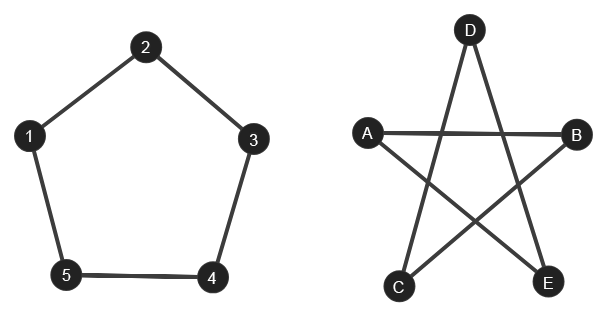
\includegraphics[width=0.9\textwidth]{iso.png}
\end{minipage}}}

Consider the language
\[GRAPH-ISO = \{\langle G, H\rangle \ | \ G \texttt{ and } H \texttt{ are isomorphic graphs}\}\]
Prove that $GRAPH-ISO \in \mathcal{NP}$.
\end{question}

\clearpage

% ------------------
% NP-Complete
% ------------------
\begin{question}{9}\textbf{$\mathcal{NP}-$complete}\\\\
Consider the following scheduling problem. You are given a list of courses $C = \{C_1,...,C_k\}$ to be scheduled into time slots. You are also given a list of students $S=\{S_1,...,S_l\}$, where each student wants to take some specified subset of these courses.\\\\
You are asked to determine whether it is possible to schedule these courses into 3 time slots (\textit{morning}, \textit{afternoon}, and \textit{evening}) such that that no student is required to take two courses in the same time slot.
\begin{enumerate}[(a)]
\item Formulate this problem as a language:\\\\
$3SCHEDULE =$
\vspace{10em}
\item Show that $3SCHEDULE \in \mathcal{NP}$ by describing a certificate (``witness'') that can be verified in polynomial time.\vfill{}\begin{center}\textit{Note: this problem continues on the next page.}\end{center}\clearpage
\item Show that $SCHEDULE$ is $\mathcal{NP}-$complete using a reduction.
\end{enumerate}
\end{question}
\clearpage

% ------------------
% BONUS
% ------------------
\textbf{Bonus Question: Theory in the Wild}\\\\
To earn a bonus point, briefly describe the key idea of \textbf{one ``Theory in the Wild'' presentation other than your own}.

% --------------------------------------------------------------
%     You don't have to mess with anything below this line.
% --------------------------------------------------------------
 
\end{document}